% Options for packages loaded elsewhere
\PassOptionsToPackage{unicode}{hyperref}
\PassOptionsToPackage{hyphens}{url}
\PassOptionsToPackage{dvipsnames,svgnames,x11names}{xcolor}
%
\documentclass[
]{article}

\usepackage{amsmath,amssymb}
\usepackage{lmodern}
\usepackage{iftex}
\ifPDFTeX
  \usepackage[T1]{fontenc}
  \usepackage[utf8]{inputenc}
  \usepackage{textcomp} % provide euro and other symbols
\else % if luatex or xetex
  \usepackage{unicode-math}
  \defaultfontfeatures{Scale=MatchLowercase}
  \defaultfontfeatures[\rmfamily]{Ligatures=TeX,Scale=1}
  \setmainfont[]{Latin Modern Roman}
  \setmathfont[]{Latin Modern Math}
\fi
% Use upquote if available, for straight quotes in verbatim environments
\IfFileExists{upquote.sty}{\usepackage{upquote}}{}
\IfFileExists{microtype.sty}{% use microtype if available
  \usepackage[]{microtype}
  \UseMicrotypeSet[protrusion]{basicmath} % disable protrusion for tt fonts
}{}
\makeatletter
\@ifundefined{KOMAClassName}{% if non-KOMA class
  \IfFileExists{parskip.sty}{%
    \usepackage{parskip}
  }{% else
    \setlength{\parindent}{0pt}
    \setlength{\parskip}{6pt plus 2pt minus 1pt}}
}{% if KOMA class
  \KOMAoptions{parskip=half}}
\makeatother
\usepackage{xcolor}
\setlength{\emergencystretch}{3em} % prevent overfull lines
\setcounter{secnumdepth}{5}
% Make \paragraph and \subparagraph free-standing
\ifx\paragraph\undefined\else
  \let\oldparagraph\paragraph
  \renewcommand{\paragraph}[1]{\oldparagraph{#1}\mbox{}}
\fi
\ifx\subparagraph\undefined\else
  \let\oldsubparagraph\subparagraph
  \renewcommand{\subparagraph}[1]{\oldsubparagraph{#1}\mbox{}}
\fi


\providecommand{\tightlist}{%
  \setlength{\itemsep}{0pt}\setlength{\parskip}{0pt}}\usepackage{longtable,booktabs,array}
\usepackage{calc} % for calculating minipage widths
% Correct order of tables after \paragraph or \subparagraph
\usepackage{etoolbox}
\makeatletter
\patchcmd\longtable{\par}{\if@noskipsec\mbox{}\fi\par}{}{}
\makeatother
% Allow footnotes in longtable head/foot
\IfFileExists{footnotehyper.sty}{\usepackage{footnotehyper}}{\usepackage{footnote}}
\makesavenoteenv{longtable}
\usepackage{graphicx}
\makeatletter
\def\maxwidth{\ifdim\Gin@nat@width>\linewidth\linewidth\else\Gin@nat@width\fi}
\def\maxheight{\ifdim\Gin@nat@height>\textheight\textheight\else\Gin@nat@height\fi}
\makeatother
% Scale images if necessary, so that they will not overflow the page
% margins by default, and it is still possible to overwrite the defaults
% using explicit options in \includegraphics[width, height, ...]{}
\setkeys{Gin}{width=\maxwidth,height=\maxheight,keepaspectratio}
% Set default figure placement to htbp
\makeatletter
\def\fps@figure{htbp}
\makeatother
\newlength{\cslhangindent}
\setlength{\cslhangindent}{1.5em}
\newlength{\csllabelwidth}
\setlength{\csllabelwidth}{3em}
\newlength{\cslentryspacingunit} % times entry-spacing
\setlength{\cslentryspacingunit}{\parskip}
\newenvironment{CSLReferences}[2] % #1 hanging-ident, #2 entry spacing
 {% don't indent paragraphs
  \setlength{\parindent}{0pt}
  % turn on hanging indent if param 1 is 1
  \ifodd #1
  \let\oldpar\par
  \def\par{\hangindent=\cslhangindent\oldpar}
  \fi
  % set entry spacing
  \setlength{\parskip}{#2\cslentryspacingunit}
 }%
 {}
\usepackage{calc}
\newcommand{\CSLBlock}[1]{#1\hfill\break}
\newcommand{\CSLLeftMargin}[1]{\parbox[t]{\csllabelwidth}{#1}}
\newcommand{\CSLRightInline}[1]{\parbox[t]{\linewidth - \csllabelwidth}{#1}\break}
\newcommand{\CSLIndent}[1]{\hspace{\cslhangindent}#1}

\usepackage{arxiv}
\usepackage{orcidlink}
\usepackage{amsmath}
\usepackage[T1]{fontenc}
\makeatletter
\makeatother
\makeatletter
\makeatother
\makeatletter
\@ifpackageloaded{caption}{}{\usepackage{caption}}
\AtBeginDocument{%
\ifdefined\contentsname
  \renewcommand*\contentsname{Table of contents}
\else
  \newcommand\contentsname{Table of contents}
\fi
\ifdefined\listfigurename
  \renewcommand*\listfigurename{List of Figures}
\else
  \newcommand\listfigurename{List of Figures}
\fi
\ifdefined\listtablename
  \renewcommand*\listtablename{List of Tables}
\else
  \newcommand\listtablename{List of Tables}
\fi
\ifdefined\figurename
  \renewcommand*\figurename{Figure}
\else
  \newcommand\figurename{Figure}
\fi
\ifdefined\tablename
  \renewcommand*\tablename{Table}
\else
  \newcommand\tablename{Table}
\fi
}
\@ifpackageloaded{float}{}{\usepackage{float}}
\floatstyle{ruled}
\@ifundefined{c@chapter}{\newfloat{codelisting}{h}{lop}}{\newfloat{codelisting}{h}{lop}[chapter]}
\floatname{codelisting}{Listing}
\newcommand*\listoflistings{\listof{codelisting}{List of Listings}}
\makeatother
\makeatletter
\@ifpackageloaded{caption}{}{\usepackage{caption}}
\@ifpackageloaded{subcaption}{}{\usepackage{subcaption}}
\makeatother
\makeatletter
\@ifpackageloaded{tcolorbox}{}{\usepackage[many]{tcolorbox}}
\makeatother
\makeatletter
\@ifundefined{shadecolor}{\definecolor{shadecolor}{rgb}{.97, .97, .97}}
\makeatother
\makeatletter
\makeatother
\ifLuaTeX
  \usepackage{selnolig}  % disable illegal ligatures
\fi
\IfFileExists{bookmark.sty}{\usepackage{bookmark}}{\usepackage{hyperref}}
\IfFileExists{xurl.sty}{\usepackage{xurl}}{} % add URL line breaks if available
\urlstyle{same} % disable monospaced font for URLs
\hypersetup{
  pdftitle={Transformer-based model to predict the outcomes of soccer matches from leagues worldwide.},
  pdfauthor={Tarak Kharrat; Meher Kharbachi},
  pdfkeywords={Transformers, Deep learning, Soccer},
  colorlinks=true,
  linkcolor={blue},
  filecolor={Maroon},
  citecolor={Blue},
  urlcolor={Blue},
  pdfcreator={LaTeX via pandoc}}

\renewcommand{\today}{3/28/23}
\newcommand{\runninghead}{A Preprint }
\title{Transformer-based model to predict the outcomes of soccer matches
from leagues worldwide.}
\author{
\textbf{Tarak Kharrat}\\R\&D Department\\Real Analytics\\\\\\\\\\
\textbf{Meher Kharbachi}\\R\&D Department\\Real Analytics\\\\}
\date{3/28/23}
\begin{document}
\maketitle
\begin{abstract}
In this work, we propose a transformer-based model for unsupervised
representation learning of multivariate time series to predict the
outcomes of soccer matches from leagues worldwide. this model is
multitask in which it predicts the 1X2 probabilities and the exact
scores ( goals scored by home and away team).
\end{abstract}
{\bfseries \emph Keywords}
\def\sep{\textbullet\ }
Transformers \sep Deep learning \sep 
Soccer

\ifdefined\Shaded\renewenvironment{Shaded}{\begin{tcolorbox}[interior hidden, sharp corners, frame hidden, borderline west={3pt}{0pt}{shadecolor}, boxrule=0pt, breakable, enhanced]}{\end{tcolorbox}}\fi

\hypertarget{introduction}{%
\section{Introduction}\label{introduction}}

Soccer is the most popular sport in the world, and predicting the
outcomes of matches has always been of great interest to sports
enthusiasts, analysts, and betting companies. Traditional methods of
prediction have relied on simple statistical models, but with the
increasing availability of data and advancements in machine learning,
more sophisticated models can be developed to improve prediction
accuracy.

\hypertarget{model-architecture}{%
\section{Model Architecture}\label{model-architecture}}

In this work, we propose a \texttt{transformer-based}(Zerveas et al.
(2021)) model for unsupervised representation learning of
\texttt{multivariate\ time\ series} to predict \texttt{soccer} match
outcomes from leagues around the world. Our model ingests team features
inputs, each containing \texttt{statistical\ performance} realised
during each played game. The model architecture consists of an
\texttt{embedding\ layer}, a \texttt{positional\ encoder}, and an
N-layer stack of \texttt{self-attention} and \texttt{feedforward}
networks. The embedding output, the feedforward network's ``Z'' vectors,
are concatenated to produce a single vector containing information on
both \texttt{home} and \texttt{away} teams. This vector is subsequently
transmitted through a \texttt{multitask} learning
\texttt{linear\ layer}, which produces two sorts of results:
\texttt{goal\ difference} and \texttt{1x2} outcome probabilities.

We evaluate the effectiveness of our model using
\texttt{negative\ log\ likelihood} losses for both \texttt{1x2} and
\texttt{goal\ difference} predictions to update the network parameters,
and we can produce the \texttt{exact\ score} of a particular game
utilising goal differences probas and \texttt{empirical\ score}
probabilities by competition.
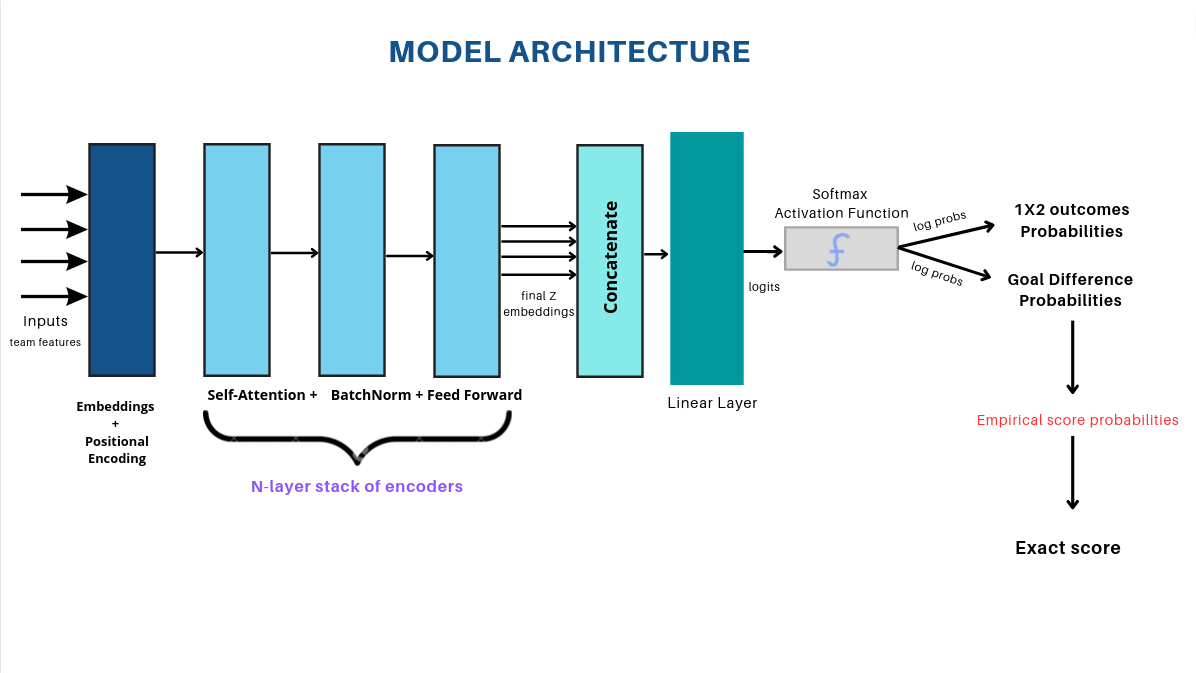
\includegraphics{figures/model_architecture.png}

\hypertarget{refs}{}
\begin{CSLReferences}{1}{0}
\leavevmode\vadjust pre{\hypertarget{ref-zerveas_transformer-based_2021}{}}%
Zerveas, George, Srideepika Jayaraman, Dhaval Patel, Anuradha
Bhamidipaty, and Carsten Eickhoff. 2021. {``A Transformer-Based
Framework for Multivariate Time Series Representation Learning.''} In
\emph{Proceedings of the 27th ACM SIGKDD Conference on Knowledge
Discovery \&Amp; Data Mining}, 2114--24. KDD '21. New York, NY, USA:
Association for Computing Machinery.
\url{https://doi.org/10.1145/3447548.3467401}.

\end{CSLReferences}



\end{document}
